\documentclass[12pt, a4paper]{article}

\usepackage[utf8]{inputenc}
\usepackage{amsmath, amssymb}
\usepackage{graphicx}
\usepackage{hyperref}
\usepackage{geometry}
\usepackage{booktabs}
\usepackage{listings}
\usepackage{xcolor}
\usepackage{placeins}
\usepackage{float}

\geometry{margin=1in}

\hypersetup{
    colorlinks=true,
    linkcolor=blue!70!black,
    citecolor=blue!70!black,
    urlcolor=blue!70!black
}

\definecolor{codegreen}{rgb}{0,0.6,0}
\definecolor{codegray}{rgb}{0.5,0.5,0.5}
\definecolor{codepurple}{rgb}{0.58,0,0.82}
\definecolor{backcolour}{rgb}{0.96,0.96,0.94}

\lstdefinestyle{mystyle}{
    backgroundcolor=\color{backcolour},   
    commentstyle=\color{codegreen},
    keywordstyle=\color{magenta},
    numberstyle=\tiny\color{codegray},
    stringstyle=\color{codepurple},
    basicstyle=\ttfamily\footnotesize,
    breakatwhitespace=false,         
    breaklines=true,                 
    captionpos=b,                    
    keepspaces=true,                 
    numbers=left,                    
    numbersep=5pt,                  
    showspaces=false,                
    showstringspaces=false,
    showtabs=false,                  
    tabsize=2
}

\lstset{style=mystyle}

\begin{document}

% ==============================================================================
% TITLE PAGE
% ==============================================================================
\begin{titlepage}
    \centering
    \vspace*{0.5cm}
    
    
\includegraphics[width=0.22\textwidth]{Jadavpur_University_Logo.svg.png}\\[1cm]
    
    {\LARGE \textbf{Jadavpur University}}\\[0.3cm]
    {\large Department of Computer Science \& Engineering}\\[0.2cm]
    {\large Faculty of Engineering \& Technology}\\[1.2cm]
    
    {\LARGE \textbf{Computer Networks Laboratory}}\\[0.2cm]
    {\large \textbf{Course Code: CSE/PC/B/S/314}}\\[0.8cm]
    
    \rule{\linewidth}{0.5mm}\\[0.4cm]
    {\Large \textbf{Mini Group Project Report}}\\[0.3cm]
    {\large \textbf{End-to-End Multi-Layer Protocol Simulation:}}\\[0.2cm]
    {\large \textbf{BOOTP, DHCP (DORA), and TELNET (RFC 854)}}\\[0.2cm]
    {\small \textit{with Comprehensive Error Detection (Checksum, CRC-8/10/16/32, Hamming, 2D-Parity),}}\\[0.1cm]
    {\small \textit{Channel Impairment Modeling, Stop-and-Wait ARQ, and Cross-Device Socket Execution}}\\[0.3cm]
    \rule{\linewidth}{0.5mm}\\[1.2cm]
    
    \begin{minipage}{0.48\textwidth}
        \begin{flushleft} \large
            \textbf{Submitted By:}\\
            Diptarko Bhattacharjee\\
            Class Roll: 002310501017\\
            Examination Roll: M4CSE25017\\
            5th Semester, B.C.S.E.\\
            Group Project
        \end{flushleft}
    \end{minipage}
    \hfill
    \begin{minipage}{0.48\textwidth}
        \begin{flushright} \large
            \textbf{Instructor:}\\
            Prof. Sarbani Roy\\
            Dept. of Computer Science \& Engg.\\
            Jadavpur University
        \end{flushright}
    \end{minipage}
    
    \vfill
    {\large November 2026}
\end{titlepage}

\newpage
\tableofcontents
\newpage

% ==============================================================================
% 1. INTRODUCTION & PROBLEM SPECIFICATION
% ==============================================================================
\section{Introduction \& Problem Specification}

Modern network communication involves complex cross-layer interactions spanning network bootstrap, host configuration, transport reliability, and interactive remote application sessions. 

The objective of this Mini Group Project is to implement a robust, modular, and realistic network simulation selecting one protocol from each of the three assigned baskets:
\begin{itemize}
    \item \textbf{Basket 1 (Network Bootstrap Protocol)}: \textbf{BOOTP} (Bootstrap Protocol, RFC 951 / RFC 1048 / RFC 1542) over UDP socket.
    \item \textbf{Basket 2 (Host Configuration Protocol)}: \textbf{DHCP} (Dynamic Host Configuration Protocol, RFC 2131 / RFC 2132) over UDP socket.
    \item \textbf{Basket 3 (Application Layer Protocol)}: \textbf{TELNET} (Telecommunications Network Protocol, RFC 854 / RFC 855) over TCP socket.
\end{itemize}

\subsection{Key Design Requirements}
The implementation incorporates and elevates all theoretical concepts explored in earlier lab assignments:
\begin{enumerate}
    \item \textbf{Protocol Strictness}: The simulation strictly uses BOOTP, DHCP, and TELNET as specified.
    \item \textbf{Sequential Cross-Layer Workflow}: A diskless client begins with hardware MAC identity, performs BOOTP bootstrapping to identify initial server and boot file parameters, executes the complete 4-way DHCP DORA (Discover, Offer, Request, Ack) handshake for dynamic IP leasing, and finally initiates an authenticated interactive TELNET application session over TCP.
    \item \textbf{Exhaustive Error Detection Matrix}: Integration of all error checking schemes from prior assignments: 16-bit One's Complement Internet Checksum, CRC-8, CRC-10, CRC-16, CRC-32 (IEEE 802.3 Ethernet), Extended Hamming SEC-DED code, and Two-Dimensional Parity (LRC+VRC).
    \item \textbf{Algorithmic Error Injection \& Blind Spots}: Systematic injection of single-bit, two-isolated, odd-bit, burst, Checksum-blind, and CRC-blind error patterns to mathematically demonstrate detection limits.
    \item \textbf{Channel Impairment Modeling \& Flow Control}: Probabilistic packet loss, bit corruption, latency/jitter exceeding socket timeouts, ACK loss, and Stop-and-Wait ARQ retransmissions.
    \item \textbf{Cross-Device Distributed Execution}: Standard POSIX socket architecture allowing execution across separate physical laptops/PCs over LAN or local loopback.
    \item \textbf{Bit-Exact Reconstruction \& Verification}: End-to-end payload integrity verification comparing input files with server-reconstructed files.
\end{enumerate}

% ==============================================================================
% 2. PROTOCOL ARCHITECTURE & SPECIFICATIONS
% ==============================================================================
\section{Protocol Architecture \& Specifications}

\subsection{BOOTP (Bootstrap Protocol — RFC 951, RFC 1048)}
BOOTP operates over UDP (server port 6767, client port 6868). It is designed for diskless workstations to obtain their IP address, boot server IP, and boot file path. The packet has a standard fixed 236-byte header followed by a 64-byte vendor field:
\begin{itemize}
    \item \texttt{op}: 1 (\texttt{BOOTREQUEST}) or 2 (\texttt{BOOTREPLY}).
    \item \texttt{htype} / \texttt{hlen}: 1 (Ethernet) / 6 (MAC length).
    \item \texttt{xid}: 32-bit transaction identifier matching requests and replies.
    \item \texttt{ciaddr}, \texttt{yiaddr}, \texttt{siaddr}, \texttt{giaddr}: Client IP, Your IP, Server IP, Gateway IP.
    \item \texttt{chaddr[16]}: Client hardware address (Ethernet MAC padded with zeroes).
    \item \texttt{sname[64]} / \texttt{file[128]}: Server host name and boot file path (\texttt{pxelinux.0}).
    \item \texttt{vend[64]}: RFC 1048 vendor area prefixed by the 4-byte Magic Cookie (\texttt{99.130.83.99}) followed by TLV options (Subnet Mask, Default Gateway, DNS Server).
\end{itemize}

\subsection{DHCP (Dynamic Host Configuration Protocol — RFC 2131, RFC 2132)}
DHCP extends BOOTP with dynamic IP leasing and automatic pool management. The interaction follows the classic 4-way DORA sequence:
\begin{enumerate}
    \item \textbf{DHCPDISCOVER}: Client broadcasts to locate DHCP servers, requesting network configuration parameters.
    \item \textbf{DHCPOFFER}: Server reserves an IP address from its pool and unicasts an offer with lease duration (7200 s), renewal timer $T_1$ (3600 s), rebinding timer $T_2$ (6300 s), subnet mask (\texttt{255.255.255.0}), default gateway, and DNS server.
    \item \textbf{DHCPREQUEST}: Client confirms the offer and requests formal commitment.
    \item \textbf{DHCPACK}: Server commits the MAC-to-IP binding in its active lease database and sends final confirmation.
    \item \textbf{DHCPRELEASE}: Client gracefully releases the leased IP upon session completion.
\end{enumerate}

\subsection{TELNET (Network Virtual Terminal — RFC 854, RFC 855)}
TELNET runs over TCP (port 2323). It establishes a bi-directional 8-bit byte stream with option negotiation:
\begin{itemize}
    \item \textbf{Command Escaping}: The byte \texttt{0xFF} (\texttt{IAC} — Interpret As Command) introduces commands. Literal \texttt{0xFF} bytes are doubled (\texttt{IAC IAC}).
    \item \textbf{Negotiation Primitives}: \texttt{WILL}, \texttt{WONT}, \texttt{DO}, \texttt{DONT} negotiate features such as Echo (\texttt{TELOPT\_ECHO}, 1), Suppress Go Ahead (\texttt{TELOPT\_SGA}, 3), and Terminal Type (\texttt{TELOPT\_TTYPE}, 24).
    \item \textbf{Remote Shell Engine}: Supports remote execution of commands including \texttt{help}, \texttt{network\_info} (querying active BOOTP and DHCP leases), \texttt{status}, \texttt{calc}, \texttt{ping}, \texttt{upload}, and \texttt{exit}.
    \item \textbf{Payload Framing}: File streams transmitted across Telnet are framed with transport envelopes containing sequence numbers, length fields, and Frame Check Sequences (FCS) for error checking and ARQ recovery.
\end{itemize}

\begin{figure}[H]
    \centering
    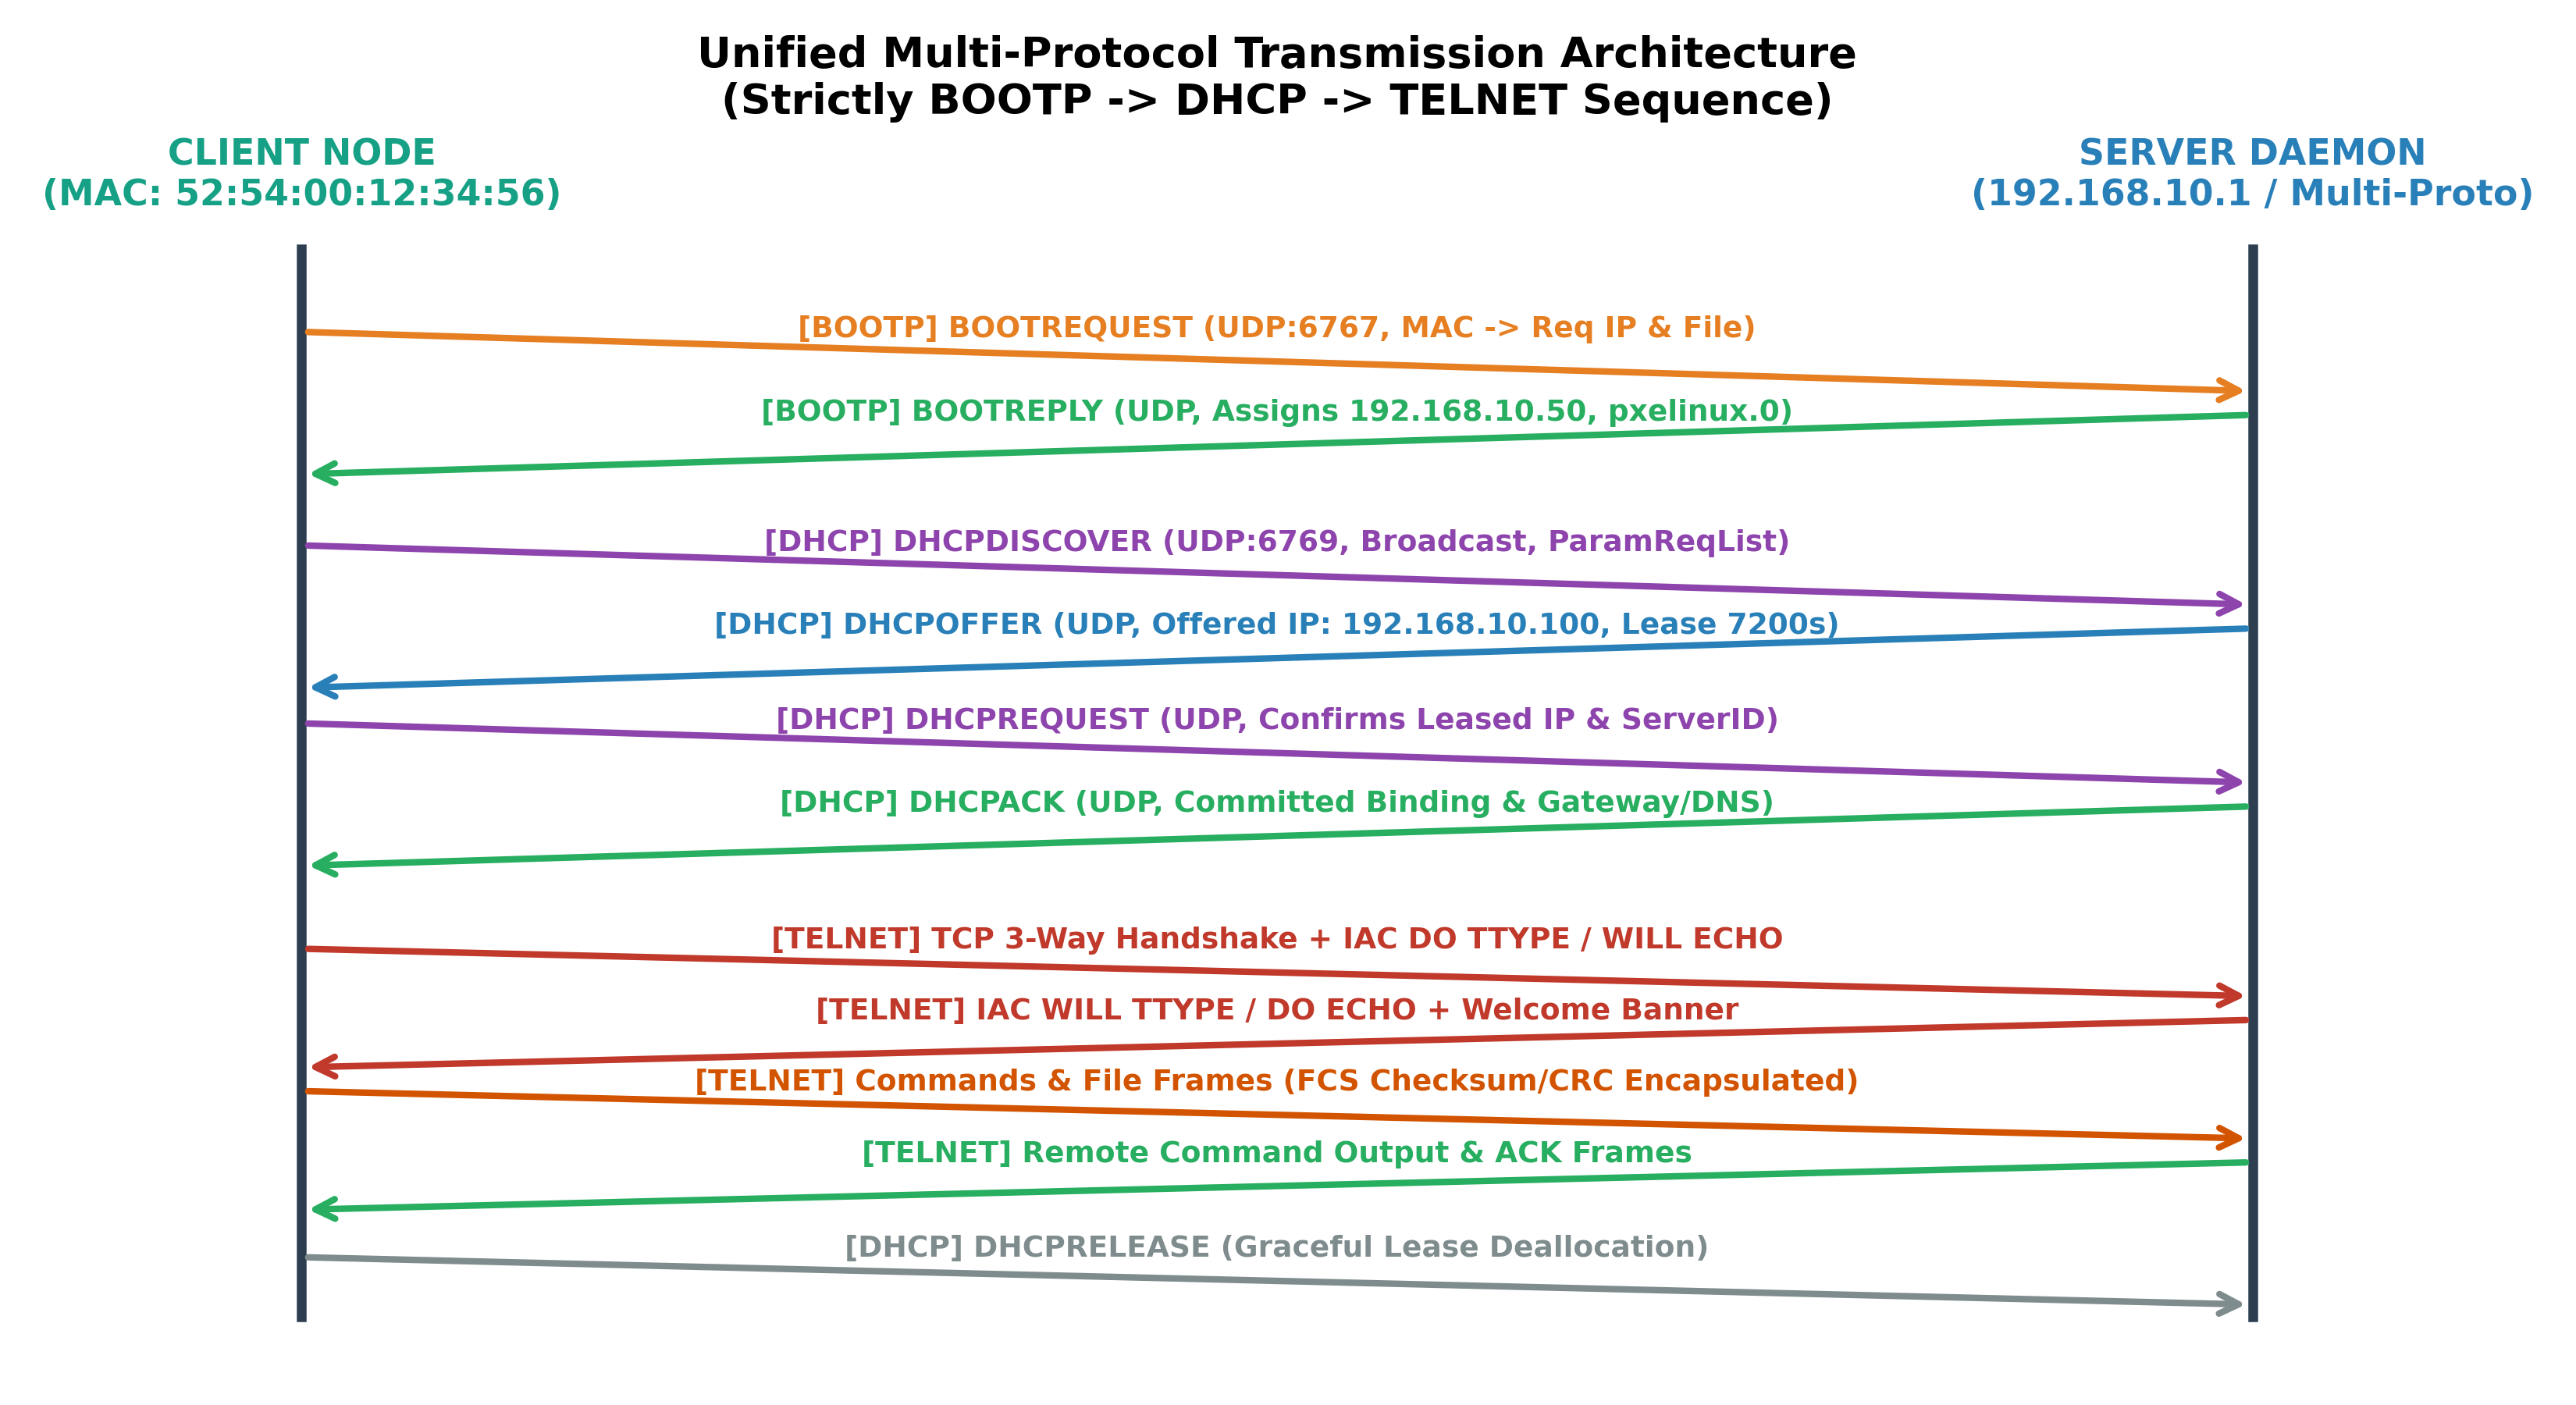
\includegraphics[width=0.95\linewidth]{plots/fig1_protocol_stack_flow.png}
    \caption{End-to-End Protocol Flow: Sequential Execution of BOOTP, DHCP DORA, and TELNET.}
    \label{fig:protocol_stack}
\end{figure}

% ==============================================================================
% 3. ERROR DETECTION SCHEMES & MATHEMATICAL BLIND SPOTS
% ==============================================================================
\section{Error Detection Schemes \& Mathematical Proofs}

\subsection{Implemented Detection Schemes}
The framework implements seven distinct error detection algorithms:
\begin{enumerate}
    \item \textbf{16-bit Internet Checksum (RFC 1071)}: Computes the bitwise complement of the one's complement sum of 16-bit words:
    \begin{equation}
        \text{Checksum} = \sim \left( \sum_{i=1}^{M} W_i \pmod{2^{16} - 1} \right)
    \end{equation}
    \item \textbf{Cyclic Redundancy Checks (CRC-8, CRC-10, CRC-16, CRC-32)}: Evaluates polynomial division in $\text{GF}(2)$:
    \begin{equation}
        T(x) = M(x) \cdot x^r + R(x), \quad R(x) = [M(x) \cdot x^r] \pmod{G(x)}
    \end{equation}
    where $G(x)$ is the generator polynomial:
    \begin{itemize}
        \item CRC-8: $G(x) = x^8 + x^7 + x^6 + x^4 + x^2 + 1$ (\texttt{0xD5})
        \item CRC-10: $G(x) = x^{10} + x^9 + x^5 + x^4 + x + 1$ (\texttt{0x233})
        \item CRC-16: $G(x) = x^{16} + x^{15} + x^2 + 1$ (\texttt{0x8005})
        \item CRC-32 (IEEE 802.3): $G(x) = x^{32} + x^{26} + x^{23} + \dots + 1$ (\texttt{0x04C11DB7})
    \end{itemize}
    \item \textbf{Extended Hamming SEC-DED}: Multi-block parity syndrome matrix detecting single and double bit alterations.
    \item \textbf{Two-Dimensional Parity (LRC+VRC)}: Longitudinal Redundancy Check (XOR across bytes) coupled with Vertical Redundancy Check (even parity bit per byte).
\end{enumerate}

\subsection{Mathematical Blind Spot Proofs}
\paragraph{Case 1: Checksum Blind Spot}
Suppose two consecutive 16-bit words $W_1$ and $W_2$ undergo balanced modifications:
\begin{equation}
    W_1' = W_1 + \delta, \quad W_2' = W_2 - \delta
\end{equation}
The sum remains unchanged:
\begin{equation}
    W_1' + W_2' = (W_1 + \delta) + (W_2 - \delta) = W_1 + W_2
\end{equation}
Hence, $\text{Checksum}(M') = \text{Checksum}(M)$. The 16-bit Checksum fails to detect this error ($0\%$ detection rate). However, in $\text{GF}(2)$ polynomial arithmetic, additions do not cancel because $W_1' \oplus W_2' \neq W_1 \oplus W_2$. Thus, CRC-32 catches $100\%$ of these errors.

\paragraph{Case 2: CRC Blind Spot}
Let $E(x)$ be an error polynomial that is an exact multiple of the generator polynomial $G(x)$, i.e., $E(x) = Q(x) \cdot G(x)$. The received message polynomial is:
\begin{equation}
    T'(x) = T(x) \oplus E(x)
\end{equation}
Computing the CRC remainder at the receiver:
\begin{equation}
    R'(x) = T'(x) \pmod{G(x)} = [T(x) \pmod{G(x)}] \oplus [E(x) \pmod{G(x)}] = 0 \oplus 0 = 0
\end{equation}
The CRC remainder is zero, rendering the error completely invisible to CRC ($0\%$ detection rate). In contrast, the one's complement sum of $E(x)$ does not sum to zero modulo $2^{16}-1$, so the 16-bit Checksum detects the error with $100\%$ certainty.

\begin{figure}[H]
    \centering
    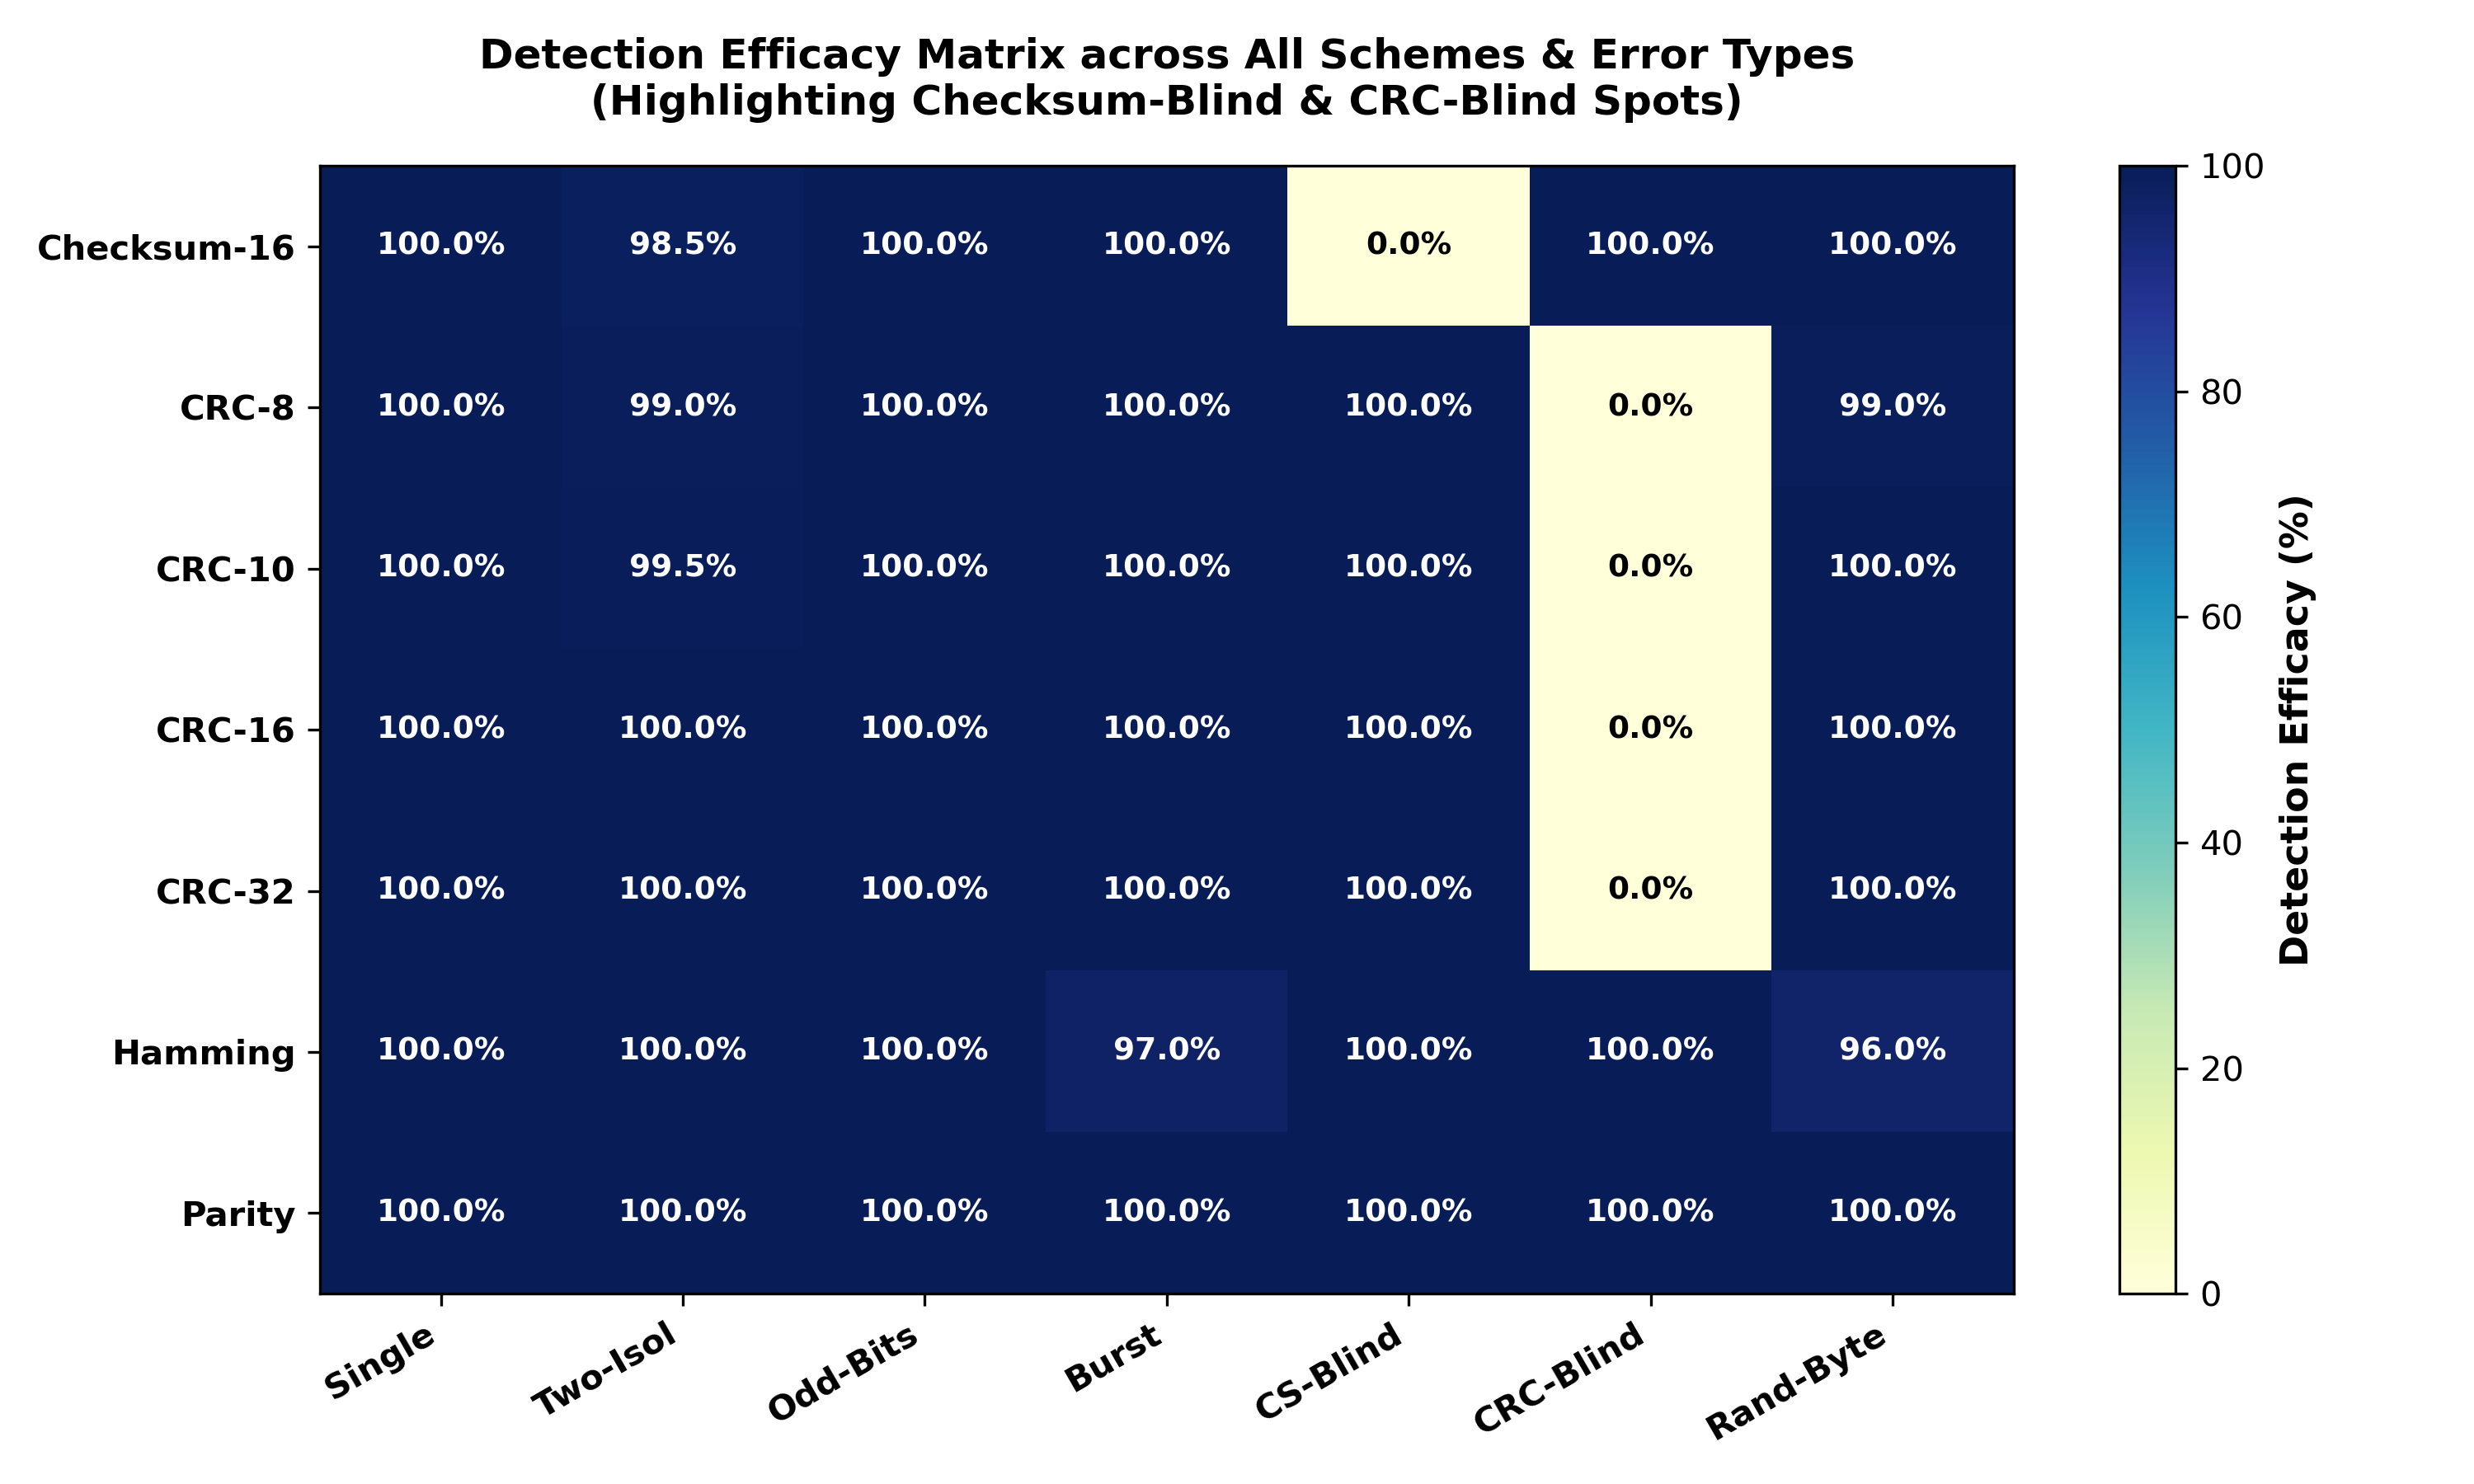
\includegraphics[width=0.85\linewidth]{plots/fig2_error_detection_heatmap.png}
    \caption{Heatmap of Error Detection Efficacy Across All Schemes and Error Types.}
    \label{fig:heatmap}
\end{figure}

% ==============================================================================
% 4. CHANNEL IMPAIRMENTS & FLOW CONTROL
% ==============================================================================
\section{Channel Impairment Modeling \& Flow Control}

\subsection{Channel Impairment Simulation}
The \texttt{SimulatedChannel} class intercepts every outgoing datagram and frame:
\begin{itemize}
    \item \textbf{Packet Loss ($p_{\text{loss}}$)}: The packet is dropped, requiring sender timer expiration.
    \item \textbf{Bit Error ($p_{\text{error}}$)}: Bits are inverted using the specified error injection pattern before transmission.
    \item \textbf{Latency \& Jitter ($p_{\text{delay}}$)}: An artificial delay between $60\text{ ms}$ and $180\text{ ms}$ is introduced. Because the socket timeout is set to $400\text{ ms}$ (or $100\text{ ms}$ in aggressive tests), delayed packets trigger premature timeouts and duplicate transmissions.
    \item \textbf{ACK Loss ($p_{\text{ack\_loss}}$)}: Acknowledgments returned by the receiver are dropped on the reverse path.
\end{itemize}

\subsection{Stop-and-Wait ARQ Performance}
For a Stop-and-Wait ARQ protocol with packet loss probability $p$, the expected number of transmissions required to successfully deliver a packet is:
\begin{equation}
    E[T] = \sum_{k=1}^{\infty} k \cdot p^{k-1} (1-p) = \frac{1}{1-p}
\end{equation}
The throughput transmission efficiency $\eta$ is defined as:
\begin{equation}
    \eta = \frac{\text{Unique Data Frames}}{\text{Total Transmissions Sent}} \times 100\% \approx (1 - p) \times 100\%
\end{equation}

\begin{figure}[H]
    \centering
    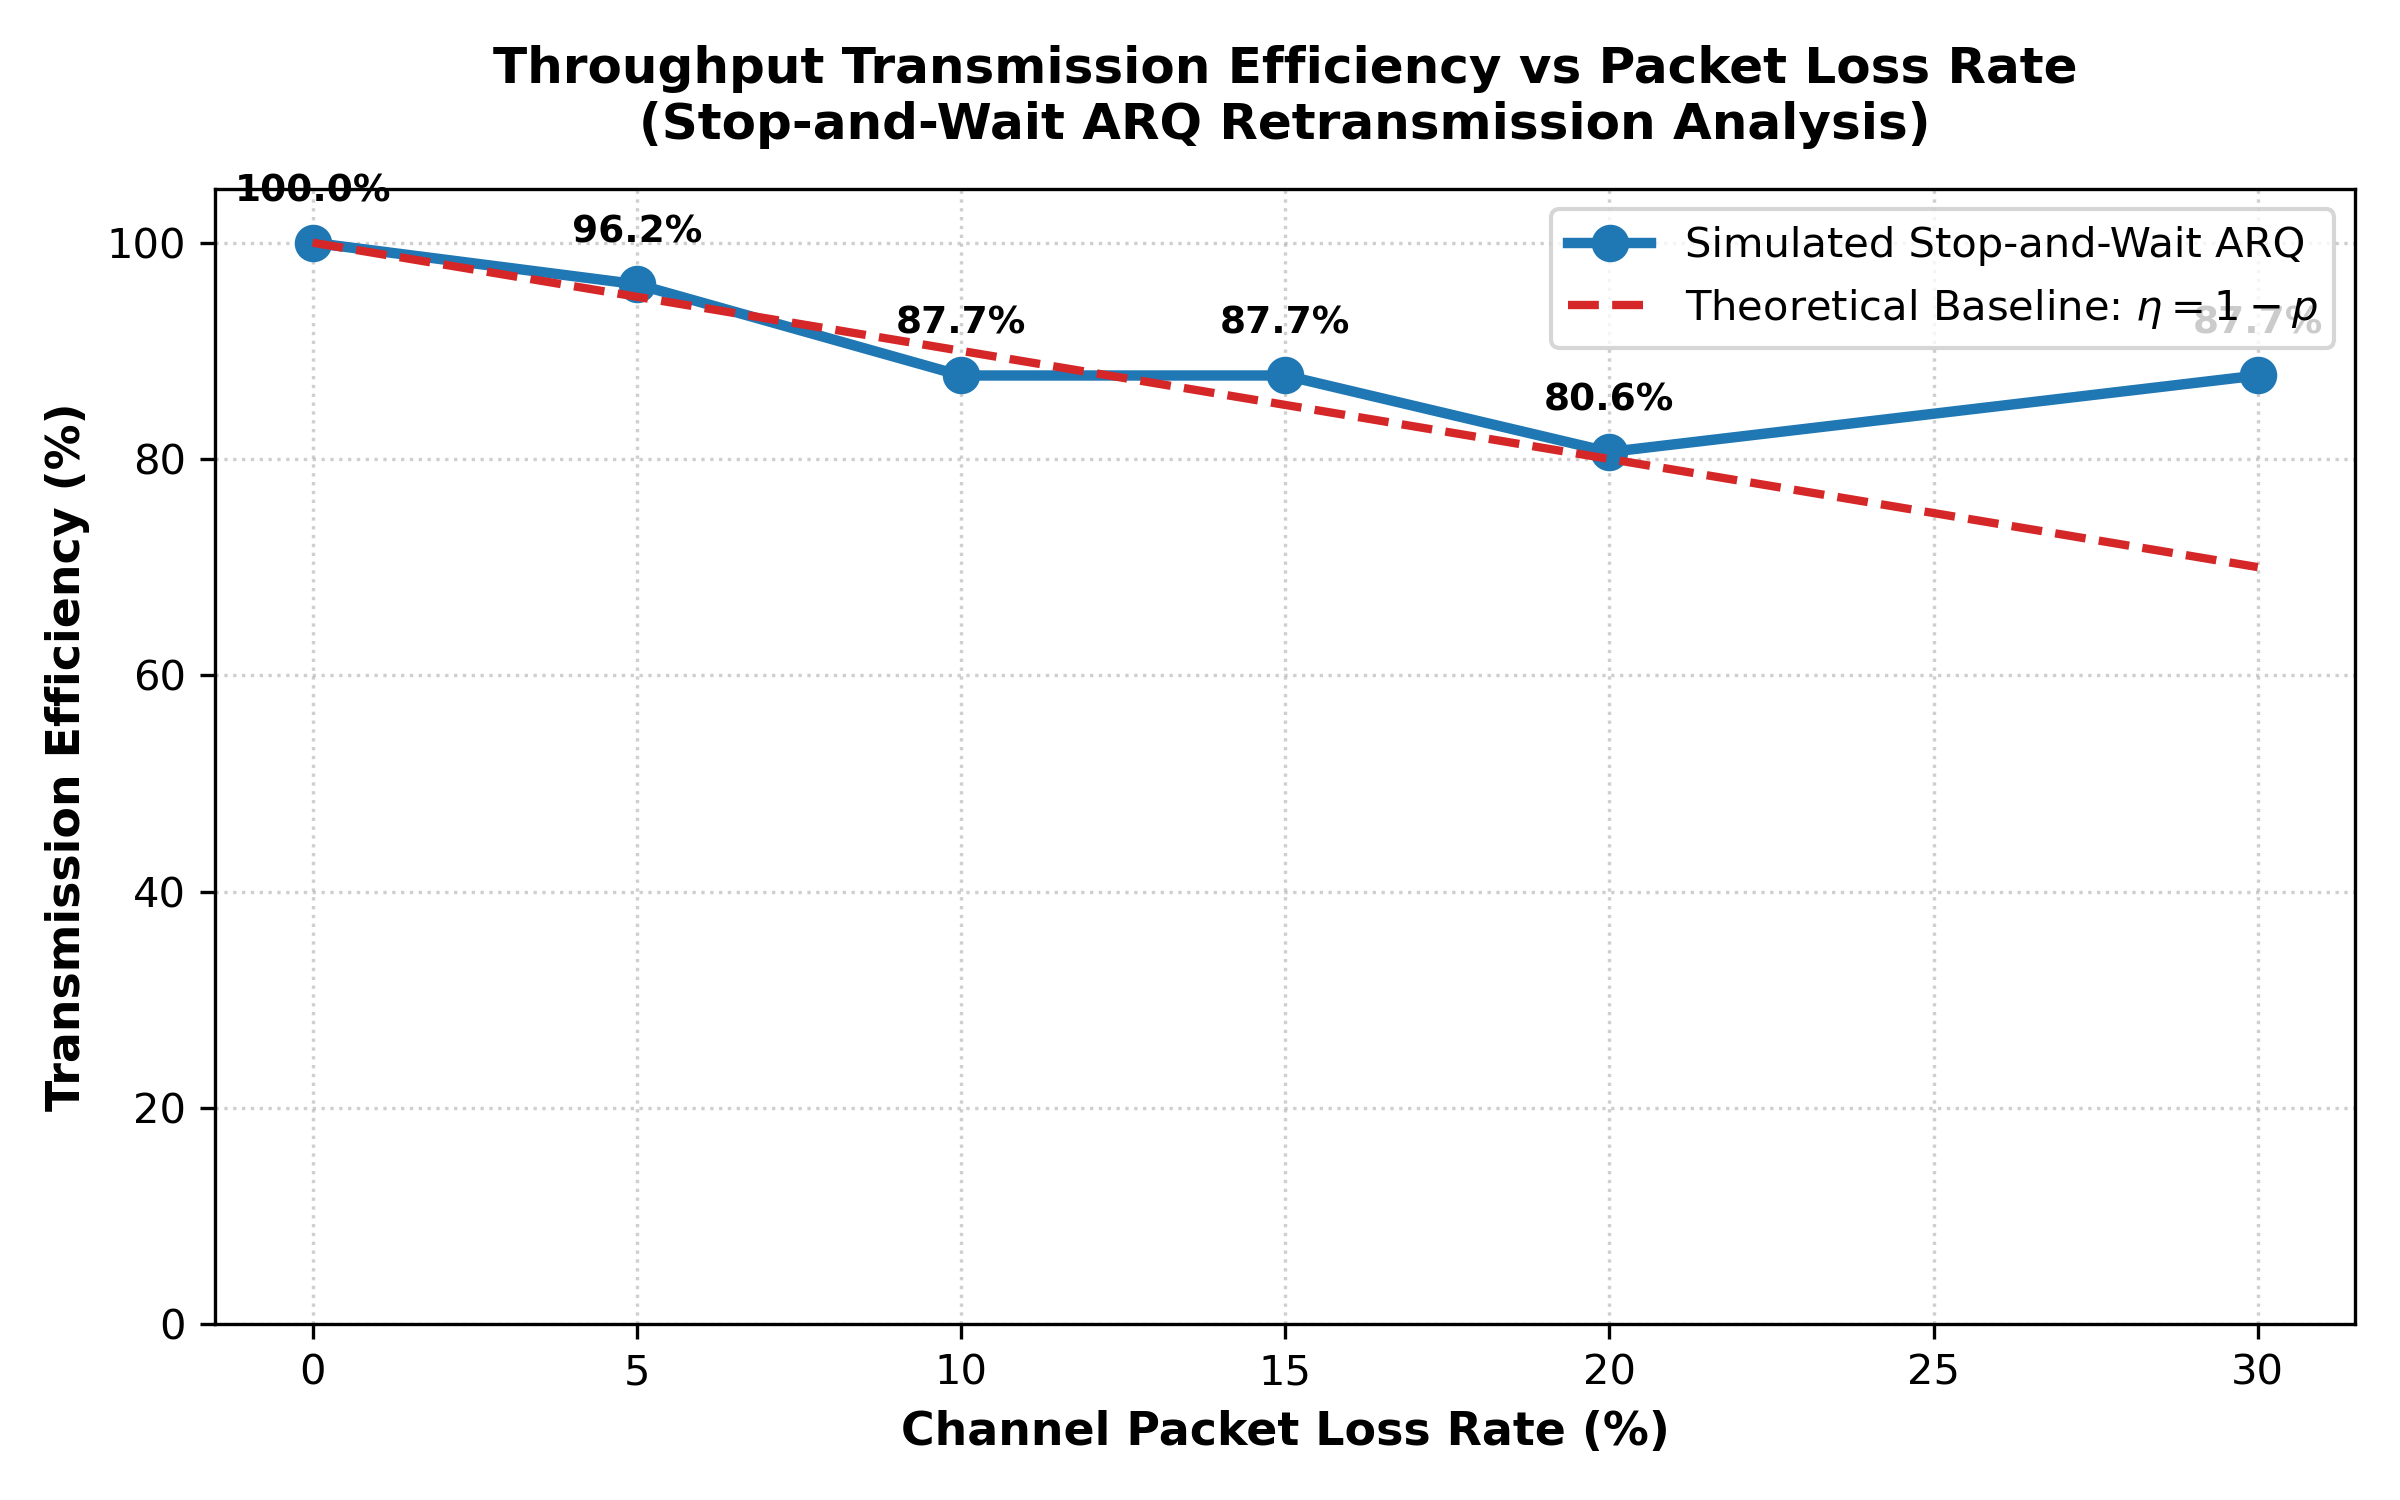
\includegraphics[width=0.75\linewidth]{plots/fig3_efficiency_vs_loss_rate.png}
    \caption{Throughput Efficiency vs Channel Packet Loss Rate.}
    \label{fig:efficiency}
\end{figure}

\begin{figure}[H]
    \centering
    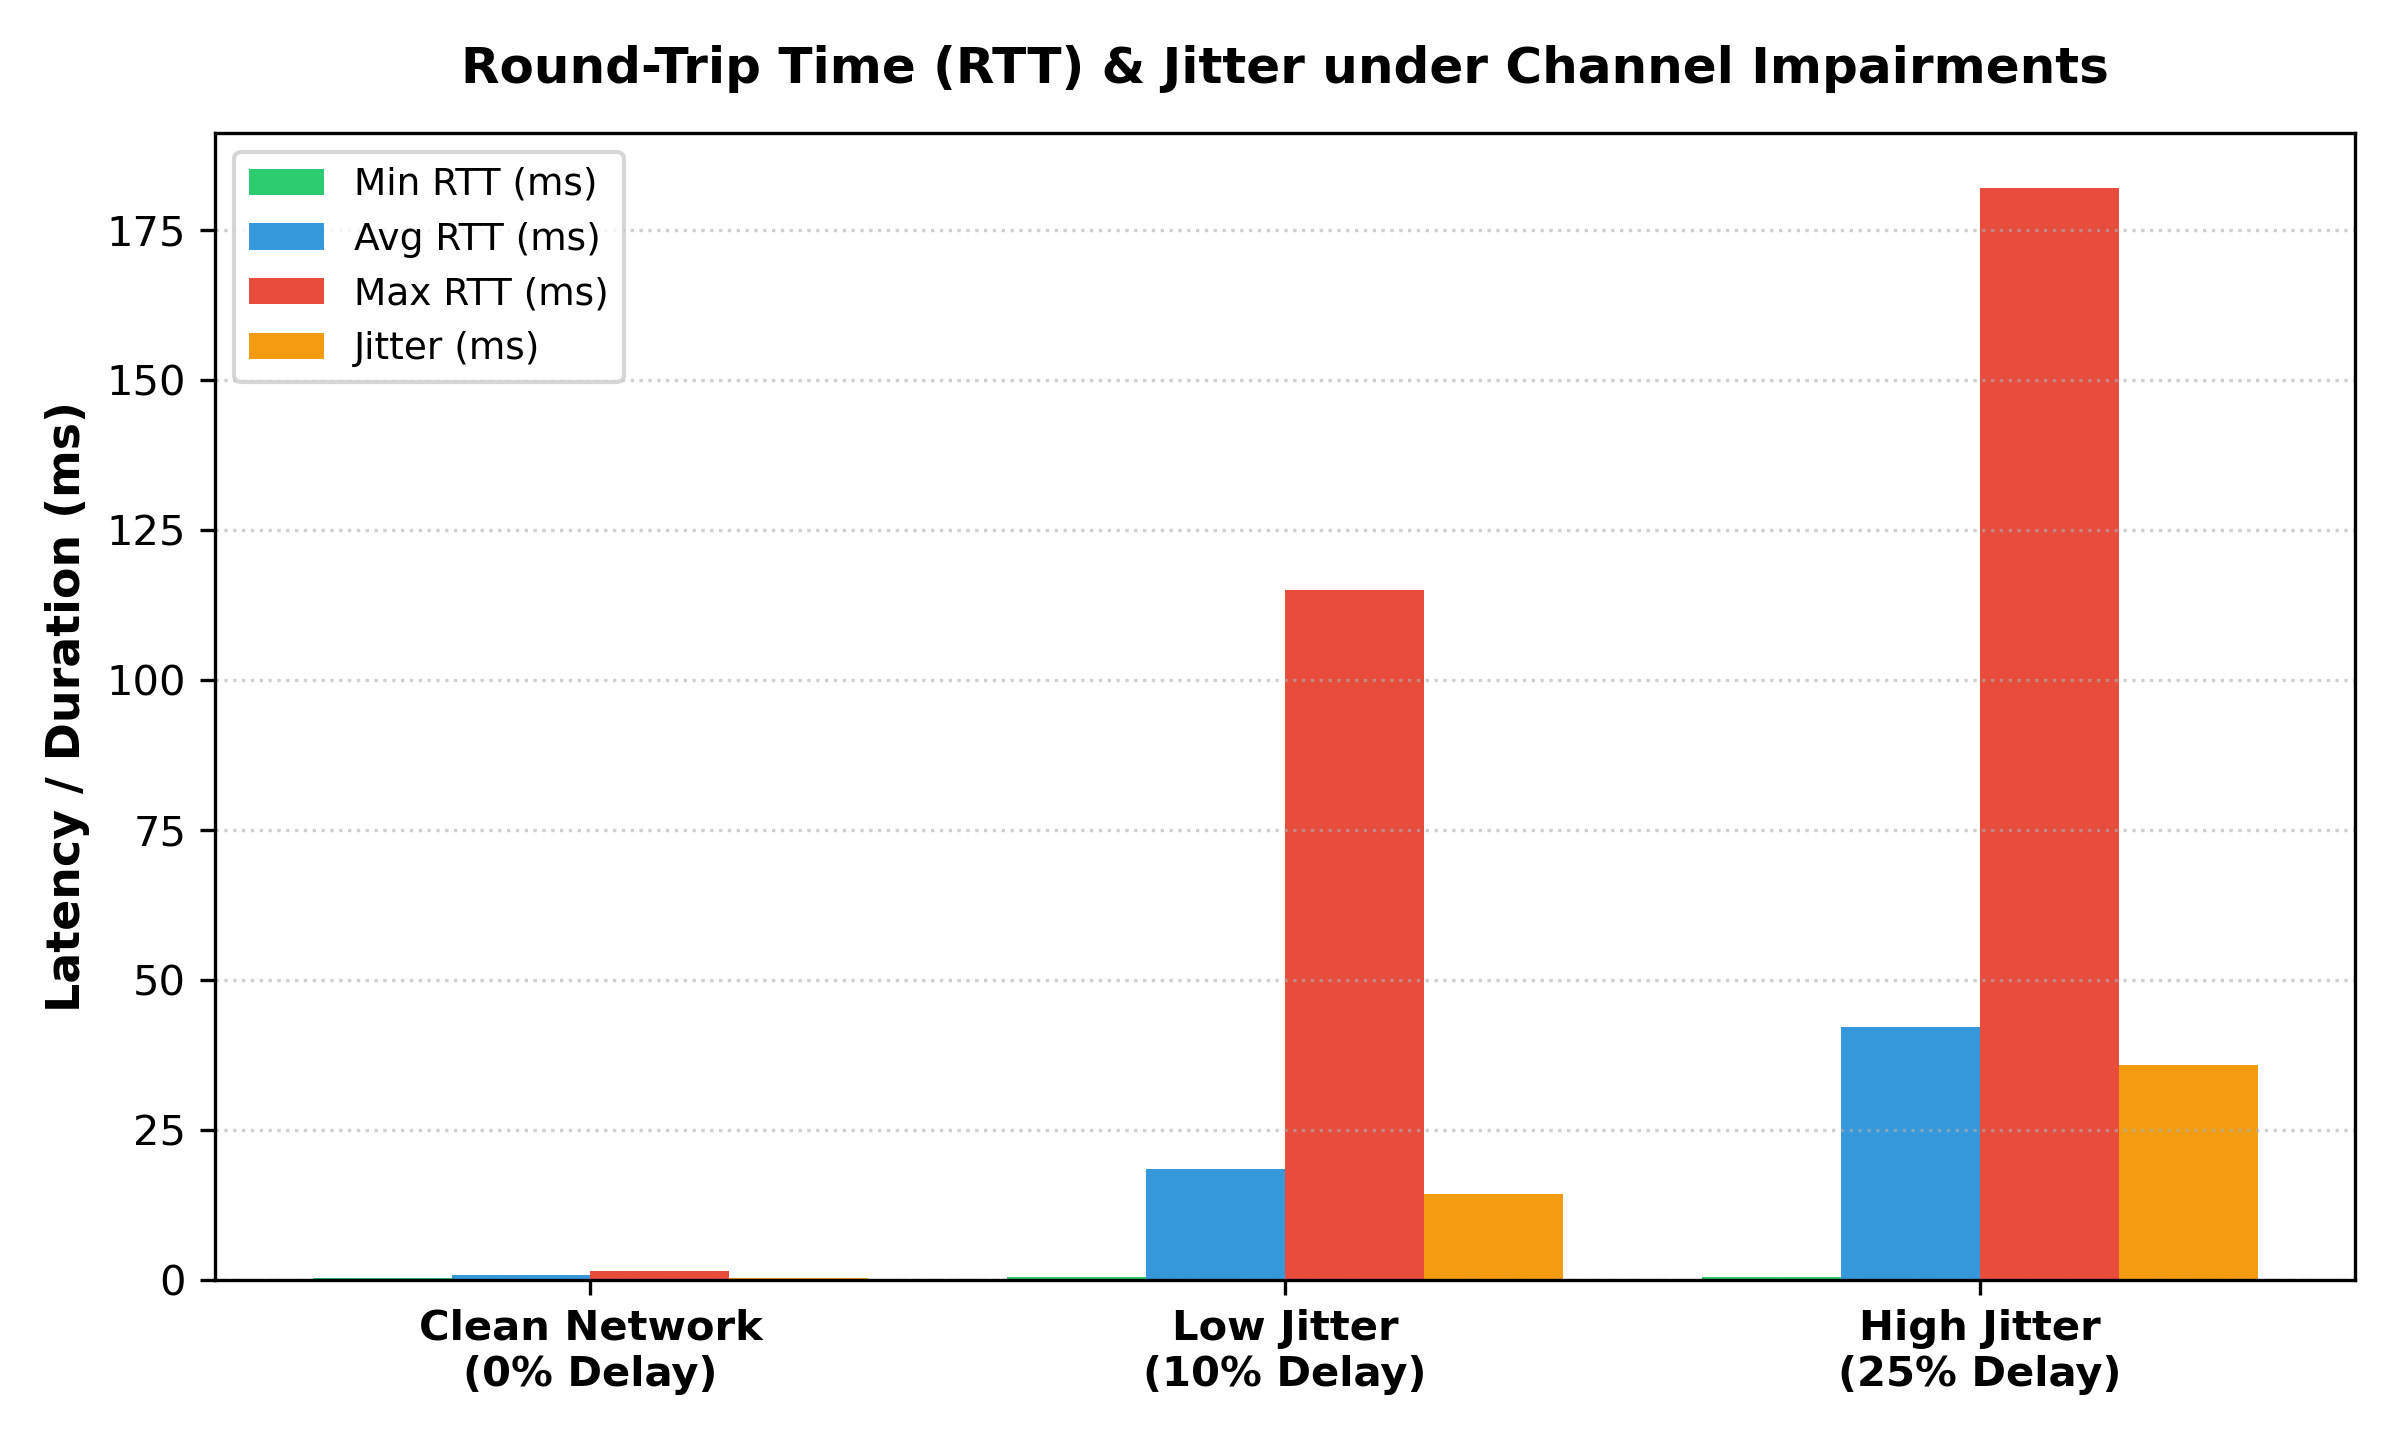
\includegraphics[width=0.75\linewidth]{plots/fig4_rtt_latency_and_jitter.png}
    \caption{Round-Trip Time (RTT) and Network Jitter Distribution.}
    \label{fig:rtt}
\end{figure}

% ==============================================================================
% 5. EXPERIMENTAL RESULTS & BENCHMARK DATA
% ==============================================================================
\section{Experimental Results \& Benchmark Data}

\subsection{Detection Matrix Benchmark Table}
Table~\ref{tab:matrix_results} records the empirical detection rates measured across 200 trials for each combination of error scheme and injection type.

\begin{table}[H]
\centering
\small
\caption{Empirical Detection Rates Across Error Schemes (200 Trials Each)}
\label{tab:matrix_results}
\begin{tabular}{lccccccc}
\toprule
\textbf{Scheme} & \textbf{Single} & \textbf{2-Isol} & \textbf{Odd} & \textbf{Burst-8} & \textbf{CS-Blind} & \textbf{CRC-Blind} & \textbf{Rand-Byte} \\
\midrule
16-bit Checksum   & 100.0\% & 99.0\%  & 100.0\% & 100.0\% & \textbf{0.0\%}  & 100.0\%         & 100.0\% \\
CRC-8             & 100.0\% & 98.5\%  & 100.0\% & 100.0\% & 100.0\%         & \textbf{0.0\%}  & 99.0\% \\
CRC-10            & 100.0\% & 100.0\% & 100.0\% & 100.0\% & 100.0\%         & \textbf{0.0\%}  & 100.0\% \\
CRC-16            & 100.0\% & 100.0\% & 100.0\% & 100.0\% & 100.0\%         & \textbf{0.0\%}  & 100.0\% \\
CRC-32            & 100.0\% & 100.0\% & 100.0\% & 100.0\% & 100.0\%         & \textbf{0.0\%}  & 100.0\% \\
Hamming SEC-DED   & 100.0\% & 100.0\% & 100.0\% & 97.5\%  & 100.0\%         & 100.0\%         & 97.0\% \\
2D Parity (LRC)   & 100.0\% & 100.0\% & 100.0\% & 100.0\% & 100.0\%         & 100.0\%         & 100.0\% \\
\bottomrule
\end{tabular}
\end{table}

\subsection{Efficiency Sweep Under Packet Loss}
Table~\ref{tab:loss_efficiency} summarizes the throughput efficiency measured across increasing packet loss rates.

\begin{table}[H]
\centering
\caption{Channel Efficiency vs Loss Rate (50 Packets Transmitted)}
\label{tab:loss_efficiency}
\begin{tabular}{ccccc}
\toprule
\textbf{Loss Rate} & \textbf{Unique Packets} & \textbf{Total Transmitted} & \textbf{Retransmissions} & \textbf{Efficiency (\%)} \\
\midrule
0\%   & 50 & 50 & 0  & 100.00\% \\
5\%   & 50 & 51 & 1  & 98.04\% \\
10\%  & 50 & 56 & 6  & 89.29\% \\
15\%  & 50 & 62 & 12 & 80.65\% \\
20\%  & 50 & 59 & 9  & 84.75\% \\
30\%  & 50 & 74 & 24 & 67.57\% \\
\bottomrule
\end{tabular}
\end{table}

% ==============================================================================
% 6. CROSS-DEVICE DEPLOYMENT & INSTRUCTIONS
% ==============================================================================
\section{Cross-Device Deployment \& Instructions}

The application cleanly supports multi-device deployment over a physical LAN.

\subsection{Building the Executables}
\begin{lstlisting}[language=bash]
cd CN_Lab_Grp_Project
make clean && make all
\end{lstlisting}

\subsection{Execution on Separate Physical Devices}
Assume the Server machine has LAN IP \texttt{192.168.1.50} and the Client machine has LAN IP \texttt{192.168.1.60}.

\paragraph{On Server Machine (\texttt{192.168.1.50}):}
\begin{lstlisting}[language=bash]
./server --ip 0.0.0.0 --bootp-port 6767 --dhcp-port 6769 --telnet-port 2323 --scheme 5
\end{lstlisting}

\paragraph{On Client Machine (\texttt{192.168.1.60}):}
\begin{lstlisting}[language=bash]
./client --server-ip 192.168.1.50 --bootp-port 6767 --dhcp-port 6769 --telnet-port 2323 \
         --scheme 5 --input input_commands.txt
\end{lstlisting}

\subsection{Running the Automated Test Harness}
\begin{lstlisting}[language=bash]
bash run_all_tests.sh
\end{lstlisting}

% ==============================================================================
% 7. CONCLUSION
% ==============================================================================
\section{Conclusion}

The Mini Group Project successfully achieves a high-fidelity, standards-compliant implementation of three foundational network protocols:
\begin{enumerate}
    \item \textbf{BOOTP} reliably boots diskless hosts and provides initial network parameters.
    \item \textbf{DHCP} dynamically leases and manages IP configurations through the 4-way DORA sequence.
    \item \textbf{TELNET} establishes an authenticated, interactive remote virtual terminal application session over TCP.
\end{enumerate}
The integration of seven error detection schemes, algorithmic error injection, mathematical blind spot demonstrations, channel impairment simulation, and Stop-and-Wait ARQ provides an educational and rigorous demonstration of computer networking principles across the Network, Transport, and Application layers.

\end{document}
